\documentclass[man,floatsintext]{apa6}
\usepackage{amsmath}
\usepackage{amssymb}
\usepackage{graphicx}
\usepackage{geometry}
\usepackage{hyperref}
\usepackage{apacite}
\usepackage{times}
\usepackage{multirow}
\usepackage{color}

\graphicspath{{images/}}

\shorttitle{Semantic coherence and distributional learning}
\title{Semantic coherence facilitates distributional learning}
\author{Long Ouyang, Lera Boroditsky, Michael C. Frank}
\affiliation{Stanford University}
\authornote{Corresponding author:\\
Long Ouyang\\
louyang@post.harvard.edu
}
\abstract{Abstract here.}


\begin{document}
\maketitle

How do people learn the meanings of words? Quine (1960) has famously observed that, based on the evidence we receive, any given word has an infinite number of logically consistent meanings. Suppose, Quine says, that we observe a foreigner utter the word \emph{gavagai} upon seeing a rabbit. There are too many consistent meanings, including ``food'', ``let's go hunting'', ``a momentary stage-rabbit'', ``undetached rabbit parts'', and so on.

One way that the hard problem of learning is softened is by a multiplicity of sources of information about word meaning. The external world, other people, and language itself provide various sources that the aspirant learner can use. Examples of informative sources include vision (Kay \& McDaniel, 1978; Rescorla, 1980; Booth \& Waxman, 2002; Regier \& Zheng, 2007), social experience (Baldwin, 1991; Bloom, 2002; Tomasello, 2003), phonology (Bloomfield, 1895; Kohler, 1929; Ramachandran and Hubbard, 2001; Maurer, Pathman, \& Mondloch, 2006; Graf-Estes et al., 2007; Parault \& Parkinson, 2008; Shukla, White, \& Aslin, 2011), syntax (Gleitman, 1990; Fisher et al., 1994), morphology (Carr \& Johnston, 2001), and linguistic context. Our chief interest in this paper is this last source -- linguistic context.

 It has long been believed that the linguistic contexts a word occurs in may be a useful clue toward its meaning. Learning from information about linguistic contexts \emph{distributional learning}. While researchers believe that distributional learning is a powerful learning mechanism, empirical results using artificial language learning suggest that human capacity for distributional learning may be quite limited.
 
In this paper, we help characterize some of the conditions under which distributional learning may succeed. Experimental work on distributional learning typically exposes learners to artificial languages where all the words are \emph{novel}. Our experiments suggest that distributional learning of meaning is facilitated by semantic coherence, the presence of \emph{known} words adhering to some semantic organization.

To preview our paper: first, we review some of the general evidence for distributional learning (readers already familiar with this literature may want to skip this section). We then introduce the specific language structure we expolore in this paper, the MNPQ language, and discuss some of successes and the failures in finding evidence of distributional learning in experiments using this language. In Experiment 1, we present evidence that semantic coherence can facilitate MNPQ learning. In Experiments 2 and 3, we further explore this effect by isolating each component of semantic coherence -- meaning and coherence -- and find that neither meaning alone nor coherence alone is sufficient to facilitate MNPQ learning. We conclude by discussing the limitations of purely artificial language learning, possibilities for future computational work, and potential mechanisms for the semantic coherence effect.

\subsection{Evidence for distributional learning}

Scholars from four separate traditions -- philosophy, linguistics, computer science, and psychology -- have suggested that people can in principle use knowledge of the linguistics contexts that a word participates as an aid to its meaning. In what follows, we briefly trace the history of this notion in each tradition.

Wittgenstein (1953/1997) was one of the first to propose that meaning derives from usage: ``for a large class of cases -- though not for all -- in which we employ the word `meaning' it can be defined thus: the meaning of a word is its use in the language'' (\S 43). In particular, Wittgenstein objected to the notion of words either as objects or as entities that could be given precise, formal characterizations. To illustrate this, he considered the word game, a term used to describe many activities, such as board games, card games, ball games, Olympic games, and so forth. These activities seem to lack a common essence that we could distill to a definition. To use a spatial metaphor, the set of things called games does not appear to be a tidy circle around which we could circumscribe a boundary, but rather a ``complicated network of similarities overlapping and crisscrossing'' (\S 66). Wittgenstein emphasized that mapping this network by describing usage was critical to understanding meaning.

Inspired by Wittgenstein, the linguist Firth proposed that people could in fact learn the meanings of words by observing their usage contexts: ``you shall know a word by the company it keeps'' (1957, p.11). Firth asserted that part of the meaning of a word is constituted by its ``habitual collocation'' (i.e., co-occurrence) with other words:

\begin{quote}
  ``The habitual collocations in which words under study appear are quite simply the word accompaniment, the other word-material in which they are most commonly or most characteristically embedded. It can safely be stated that part of the `meaning' of \emph{cows} can be indicated by collocations as \emph{They are milking the cows}, \emph{Cows give milk}. The words tigresses or lionesses are not so collocated and are already clearly separated in meaning at the collocational level'' (p12)
\end{quote}

Firth stressed the utility of \emph{pure} co-occurrence independent of extralinguistic or even grammatical aspects. He even outlined a prescient method of collocational analysis that is well describes how modern-day statistical approaches to meaning work:
\begin{quote}
  ``In the study of selected words, compounds and phrases in a restricted language for which there are restricted texts, an exhaustive collection of collocation will suggest a small number of groups of collocations for each word studied. The next step is the choice of definitions for meanings suggested by the groups'' (p13)
\end{quote}

Harris, a contemporary of Firth's, advanced a quantitative version of this notion called the \emph{distributional} hypothesis, which proposes that words are semantically similar to the degree that they participate in the same ``environments'' (1951). Harris defined the environment of a word to be the other words ``before, after, and simultaneous with the element [word] in question'' (1951, pp.16). He posited that word meanings could be compared via their distributions, or the sum of all environments that they occurred in. He believed that even in cases where word meaning was largely given by extralinguistic influences, such influences would have distributional correlates\footnote{``... it frequently happens that when we do not rest with the explanation that something is due to meaning, we discover that it has a formal regularity or `explanation.' It may still be `due to meaning' in one sense, but it accords with a distributional regularity.'' (1970, p.785)} so that meaning could be divined by rigorous quantitative analysis of linguistic contexts. Thus, he strongly advocated for statistical methods, but this vision did not come to light for some time, in part due to the rise of Chomsky's generative linguistics, which downplayed statistical approaches.

% - (transition: ideas from structural linguistics revived by computer scientists) computational models. HAL, LSA (diagrams), word classification: RCF98, Cartwright + brent, 1996, mintz et al., 2002, topic models. (bottom line: computational proof of concept)
Firth and Harris' calls for quantitative analysis went largely unheeded for the next 30 years (but see Rubenstein \& Goodenough, 1965; Clark, 1968; Geffroy et al., 1973; Stefflre, Reich, \& Stefflre, 1971; Berry-Rogghe, 1973; Jones \& Sinclair, 1974; Szalay \& Bryson, 1974). It was in the early 1980's that computer scientists revived the distributional hypothesis. Motivated by practical issues in the field of information retrieval, they considered the relationships between words themselves and between words and documents. A typical problem was that retrieving relevant documents from a database in response to a query with certain search terms. One solution to this problem is to representing documents as points in a high dimensional space whose dimensions are frequencies for different words (Salton \& McGill, 1983). This approach lends itself quite naturally to a matrix representation with words as rows, columns as documents, and particular cells encoding the frequency with which a particular word occurs in a particular document (see Figure \ref{matrix-word-doc}).

%% HT http://tex.stackexchange.com/a/2442 for the \newline method
%% to get multi-line cells. note the use of p{4cm} in the tabular
%% options
\begin{figure}
  \begin{center}
    \caption{Word-document matrix}
    \label{matrix-word-doc}

    \begin{tabular}{| l | p{4cm} | p{4cm} | l |}
      \hline
      & Document X & Document Y & ... \\
      \hline
      Word A & Frequency of word A \newline in document X & Frequency of word A \newline in document Y & ... \\
      \hline
      Word B & Frequency of word B \newline in document X & Frequency of word B \newline in document Y & ... \\
      \hline
      ... & ... & ... & ... \\
      \hline

    \end{tabular}
  \end{center}
\end{figure}

While such matrices can be interpreted as representing documents in terms of their constituent words, they can also be interpreted as representing words in terms of their patterns of use across documents, or, a proxy for the linguistic contexts that a word participates in. Put another way, such a matrix can be thought of either as a model of document meaning or -- more importantly, for our purposes -- a model of word meaning. 

Another approach was to represent words in terms of their surrounding words, which immediately affords a model of word meaning (Church \& Hanks, 1990; Schutze, 1992). In this approach, the corresponding matrix has words as both rows and columns, with frequency of co-occurrence between words occupying the cells (see Figure 2). An additional parameter is the window size -- the number of surrounding words that should be constitute a word's context.

\begin{figure}
  \begin{center}
    \caption{Word-word matrix}
    \label{matrix-word-word}

    \begin{tabular}{| l | p{3.5cm} | p{3.5cm} | p{3.5cm} | l |}
      \hline
      & Word X (-1) & Word X (+1) & Word X (+2) & ... \\
      \hline
      Word A &
      Frequency of X \newline 1 word before \newline  A &
      Frequency of X \newline 1 word after \newline  A & 
      Frequency of X \newline 2 words after \newline  A & 
      ... \\
      \hline
      Word B &
      Frequency of X \newline 1 word before\newline  B &
      Frequency of X \newline 1 word after \newline  B & 
      Frequency of X \newline 2 words after \newline  B & 
      ... \\
      \hline
      ... & ... & ... & ... & ... \\
      \hline

    \end{tabular}
  \end{center}
\end{figure}

Though these formalisms arose in response to applied computational problems, their psycholinguistic significance was not lost on the early information retrieval pioneers. Researchers began explore how these representations might support language learning, a direction that proved to be widely influential.

As one example, Landauer and Dumais (1997) developed a model called Latent Semantic Analysis (LSA), which operates on a word-document matrix. LSA applies a dimensionality reduction technique -- singular value decomposition -- to this matrix, yielding a reduced space that represents the semantic structure of the input. Each word is then associated with a vector in this reduced space and the similarity between two words can be computed as the cosine of the angle between their two vectors. The authors trained LSA on a corpus of 4.6 million words of text from encyclopedia articles and subsequently tested the model on 80 items from a Test of English as a Foreign Language (TOEFL) synonym test. They found that LSA closely matched performance of non-native English speakers applying to U.S. colleges. 

As another example, Lund and Burgess (1996) developed a model called Hyperspace Analogue to Language (HAL), which operates on a word-word matrix where co-occurrence frequencies are weighted according to the separation distance between words. Like LSA, HAL applies dimensionality reduction to this matrix, in this case removing all but the 200 highest variance columns. On a large corpus of Usenet data, HAL successfully extracted semantic categories like animals, body parts, and geographical regions. Lund and Burgess also found that distances between words in HAL space correlated positively (up to $r$=0.35) with semantic-priming reaction times.

The success of early models like HAL and LSA led to a proliferation of models that use co-occurrence information to learn word meaning (see Riordan \& Jones, 2010 for an overview and comparison of state-of-the-art models) as well as other linguistic properties like syntactic category. The computational evidence is quite strong: statistical patterns of co-occurrence can, in principle, be used to learn some aspects of word meaning.

We have computational proofs of concept? Do humans actually accomplish these behaviors? Empirical research on knowledge of visual and color terms in the congenitally blind offers some indirect evidence. Shepard and Cooper (1992), had blind, color-blind, and normally sighted participants rate the similarity of pairs of colors words. As might be predicted, the ratings of blind participants did not correlate highly with normally sighted individuals. However, their ratings did appear to preserve the local similarity relationships -- violet was rated most similar to purple, teal to green, and so forth. How might congenitally blind individuals have learned anything about color relationships? One possibility, raised by Shepard and Cooper, is that the blind may have extracted these relationships from their linguistic input. Similarly, more recent work by Bedny et al. (2011) suggests that visual verb meanings are unaffected by congenital blindness. % http://mindmodeling.org/cogsci2012/papers/0471/index.html

These demonstrations in the blind, while suggestive, are only indirect evidence of distributional learning. Researchers studying distributional learning of syntactic categories (as opposed to word meanings) have employed methods that in principle can provide stronger evidence. These studies expose learners to artificial languages with certain distributional regularities and measure whether learners form categories on the basis of these regularities. In the next section, we discuss results of studies that have examined one kind of distributional structure known as the MNPQ language.

\subsection{A puzzle: the MNPQ language}

The MNPQ language contains four categories of words, M, N, P, and Q, and sentences that subjects hear take one of two forms, MN and PQ. Early investigations (Braine, 1966; Smith, 1966) found that subjects tend to endorse novel but grammatical MN and PQ sentences as having come from the language they heard. However, subjects also endorse ungrammatical MQ and PN sentences, suggesting that they learn position regularities (that M/P come first and N/Q come second) but not co-occurrence regularities (that M co-occurs with N but not Q and that P occurs with Q but not N). This failure to learn categories (either syntactic or semantic) on the basis of pure co-occurrence has been reliably observed in a number of studies (Braine, 1987; Brooks et al., 1993; Frigo \& McDonald, 1998; Kempe \& Brooks, 2001; Gerken, Gomez \& Wilson, 2005; Lany \& Saffran, 2010; Frank \& Gibson, 2011). These results are puzzling, given that computational models strongly indicate that information sufficient for categorization exists in the linguistic input.

However, many of same these studies have also demonstrated that MNPQ learning is possible when distributional information is partially or completely correlated with another cue. For example, Braine (1987) found that successful MNPQ learning results when distributional information is partially correlated with natural gender. In this experiment, subjects acquired an artificial language by learning to name pictures of referents. In the experimental condition, all pictures of men were labeled by Ms (though not all Ms referred to men) and all pictures of women were labeled by P words (though not all Ps referred to women). Learning of the co-occurrence regularities was significantly higher in the experimental condition than in a control condition where natural gender was not correlated with M/P membership. Though Braine's experiment combined distributional cues with natural gender, he suggested that phonological cues might better serve real-world language learners. For instance, Spanish and Italian speakers might learn grammatical gender categories by taking advantage of the fact that feminine nouns often end with \emph{-a}, while masculine nouns often end with \emph{-o}.

Recently, this suggestion received attention in the work of Lany and Saffran (2010), who found that 22-month old infants successfully learned MNPQ when distributional regularities were aligned with the number of syllables in a word (in particular, when N words were disyllabic and Q words were monosyllabic) but \emph{not} when the number of syllables was not predictive of N/Q membership. These demonstrations that distributional information may be useful to the learner when combined with other information sources has motivated research on how disparate information sources might be integrated to facilitate learning (e.g., Monaghan, Chater, \& Christiansen, 2005; Johns \& Jones, 2011).

In this paper, we add to this literature by exploring a new information source: semantic coherence. All of the studies referenced above were conducted using the artificial language learning paradigm. Thus, at the beginning of the experiments, learners did not know the meanings of any of the words. Real learners, by contrast, typically know the meanings of some (if not most) words they hear and such words tend to relate to a single topic of discourse. Put another way, the language that real learners encounter tends to have semantic coherence; some words are known and adhere to some semantic organization. We ask: does semantic coherence facilitate distributional learning?

To explore this possibility, we presented subjects with an MNPQ language where sentences took the form ``M and N'' or ``P and Q''. We hypothesized that distributional learning for N and Q words would be afforded, given a certain level of semantic coherence (specifically, a taxonomic coherence where M's are animals and P's were vehicles). For instance, hearing the four sentences ``cat and dax", ``cat and ziv'', ``car and wug'', and ``car and pif'' might allow learners to infer that daxes and zivs belong to the same category, as both words co-occur with ``cat'', and that wugs and pifs belong to the same category, as both words co-occur with ``car''.

In Experiment 1, we tested whether semantic coherence facilitated distributional learning. In Experiments 2 and 3, we compared semantic coherence to phonological coherence and semantic incoherence, the presence of known words that do not adhere to some semantic organization.

\section{Experiment 1: Semantic coherence}

In all the experiments reported in this paper, we presented subjects with auditory sentences from an MNPQ language. In different conditions, we varied properties of the M's (which co-occur with N's) and P's (which co-occur with Q's). We will call the M's and P's \emph{context words}. We measured learning for the N's and Q's, which we will call the \emph{target words}.

In Experiment 1, we parametrically varied two independent properties of the context words. First, we manipulated semantic coherence -- the fraction of M/P words obeying a taxonomic organization (M = animal words, P = vehicle words). Second, as one hallmark of statistical learning is sensitivity to the amount of evidence observed, we manipulated the amount of exposure to the language.

After subjects were exposed to the language, we tested them on three measures of MNPQ learning -- sentence memory, similarity rating, and a referent assignment task.

\subsection{Method}

\subsubsection{Subjects}
678 Amazon Mechanical Turk (MTurk) workers. Using MTurk's worker qualifications, we limited participaton to workers located in the United States and with a previous HIT approval rate greater than or equal to 90\%. We chose MTurk workers because the number of experimental conditions required a large number of subjects.

\subsubsection{Materials}
Sentences took the form ``M and N'' or ``P and Q'' (see Figure \ref{mnpq-table}). Note that sentences literally included the word ``and'' in the middle. We generated the actual lexical items randomly for each subject. N's and Q's were always novel nonsense words and were drawn without replacement from the set \{moke, thite, jiv, pif, dex, wug\}. M's and P's could be either novel or familiar. Novel M's were drawn from \{feeb, bim, lup\} and novel P's were drawn from \{zabe, vap, chuv\}. Familiar M's and P's obeyed a taxonomic organization -- familiar M's were drawn from \{hamster, cat, dog\} and familiar P's were drawn from \{car, bus, truck\}. To create the audio files, we input the sentences as ``X. and. Y.'' (e.g., ``car. and. chuv.'', including periods) into an American English text-to-speech engine using a female voice\footnote{\label{tts}In particular, we programatically submitted all of the text sentences to the text-to-speech web service that powers Google Translate; when we performed the synthesis in 2011, this web service provided an excellent synthesis engine. However, the available voices have changed since then. See also Footnote \ref{change-of-stimuli}.}. The periods between words introduced substantial pauses ranging in length from 150 to 300 ms; piloting revealed that without pauses, it was difficult for participants to distinguish the words. Sentences using only monosyllabic words were around 2 seconds long. Sentences using the sole disyllabic word, hamster, were around 3 seconds long.
The referent assignment task involved visual referents. For the context words, we used 128x128 pixel images of a cat, dog, hamster, car, bus, and truck. For the target words, we used 100x100 pixel images of a horse, rabbit, sheep, bear, goldfish, mouse, boat, van, train, motorcycle, plane, and bicycle.

\begin{figure}[t]
  \begin{center}
  \caption{The MNPQ language. Underlined sentences were withheld from exposure.}
  \vskip 0.12in
  \fbox{\label{mnpq-table}
    \begin{tabular}{ l  l  l | l l l }
      \underline{$m_1$  $n_1$} & $m_1$  $n_2$ & $m_1$  $n_3$ &  \underline{$p_1$  $q_1$} & $p_1$  $q_2$ & $p_1$  $q_3$ \\
      $m_2$  $n_1$ & \underline{$m_2$  $n_2$} & $m_2$  $n_3$ &  $p_2$  $q_1$ & \underline{$p_2$  $q_2$} & $p_2$  $q_3$ \\
      $m_3$  $n_1$ & $m_3$  $n_2$ & \underline{$m_3$  $n_3$} &  $p_3$  $q_1$ & $p_3$  $q_2$ & \underline{$p_3$  $q_3$}\\
    \end{tabular}}
  \end{center}
  \vspace{-2ex}
\end{figure}

\subsubsection{Design and Procedure}

We parametrically varied coherence. The language for a subject contained either 0/3, 1/3, 2/3, or 3/3 familiar M and P words each. We also varied the amount of exposure to the language -- subjects heard either 56, 126, 196, or 392 sentences. Before starting the experiment, we asked subjects to turn on their speakers and click a button, which played a spoken English word (``airplane''). Subjects were required to correctly type the word to continue. The experiment had four phases -- exposure, similarity, memory, and referent assignment. Below, we detail these phases (for exposition, we have switched the order of memory and similarity).

\paragraph{Exposure}
Subjects listened to sentences from the language. We withheld 
six sentences from exposure (see Figure~\ref{mnpq-table}), yielding 14 unique sentences in the exposure set. Each sentence was heard either 4, 9, 14, or 28 times, giving 56, 126, 196, or 392 total trials. We presented the sentences in random order subject to the constraint that there were no repeated words between consecutive trials (pilot testing suggested that repeated words between trials substantially afforded learning). To encourage compliance, subjects had to click a button to hear each sentence.

\paragraph{Memory}
Subjects listened to sentences and judged on a 5 point scale how confident they were that they had previously heard the sentence during exposure. We tested four types of sentences:

\begin{itemize}
\item \emph{Familiar} sentences heard during exposure.
\item \emph{Withheld} sentences not heard during exposure but conforming to the MNPQ structure.
\item \emph{Cross-category} sentences of the form MQ and PN.
\item \emph{Position-violation} sentences of the form MM, NN, PP, and QQ.
\end{itemize}

Sentences were presented in random order such that there were no repeated words between consecutive trials. In two catch trials\footnote{In early runs of the experiment, we did not include catch trials. 
  Let [A/3;B] denote the experimental condition with A/3 coherence and B exposures (e.g., [2/3;196] refers to the 2/3 coherence level with 196 exposures). In [0/3;196], 18 out of 40 subjects did not receive catch trials. In [3/3;56], 30 out of 43 subjects did not receive catch trials. In [3/3;126], 30 out of 40 subjects did not receive catch trials. In [3/3;196], 30 out of 40 subjects did not receive catch trials.}, instead of a sentence from the MNPQ language, we played a non-repeatable audio instruction to press a specific response button.  If subjects learned the MN and PQ co-occurrence relationships, then we expected that they would rate novel grammatical sentences as more familiar than the cross-category sentences.

\paragraph{Similarity}
For each pair of words in the union of N and Q, we asked subjects to rate on a 5 point scale how similar they believed the two words to be in meaning. This resulted in within-category judgments (e.g., $n_1$ vs. $n_2$) and cross-category judgments (e.g., $n_1$ vs. $q_1$).	We presented the pairs in a fixed pseudorandom order containing no repeated words between consecutive trials. Though exposure was entirely auditory, for convenience, we presented these similarity questions as text (e.g., ``How similar are \textbf{pif} 
\includegraphics[width=0.3cm]{play.png} and \textbf{thite} 
\includegraphics[width=0.3cm]{play.png} ?''); to facilitate mapping between visual and spoken word forms, the speaker button next to each word played the spoken word when clicked. In two catch trials, subjects were asked to press the response button corresponding to the solution of a simple arithmetic problem. If subjects learned the MN and PQ co-occurrence relationships \emph{and} used these relationships as a basis for lexical categorization, then we expected that within-category pairs of words would be judged to be more similar than cross-category pairs.

\begin{figure}[ht]
\begin{center}
  \caption{The referent assignment task.}
  \label{meaning-task}
  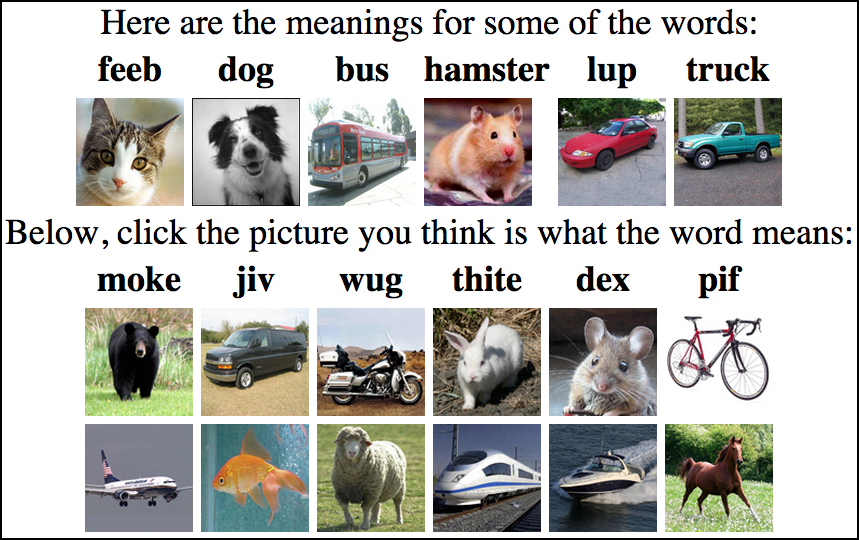
\includegraphics[width=8.5cm]{meaning-html-cropped.png}
\end{center}
\end{figure}

\paragraph{Referent assignment}
Subjects made 2AFC referent assignments for the N and Q words (see Figure~\ref{meaning-task}). At the top of the screen, we displayed the M and P words in random order. Under each word, we showed an image of an associated referent. The referents corresponded to the familiar pools for M and P words: \textsc{cat}, \textsc{dog}, \textsc{hamster}, \textsc{car}, \textsc{bus}, and \textsc{truck}. Familiar words were always associated with the obvious referents (e.g., ``dog'' was always paired with an image of a dog). Below the ``seeded'' word meanings, we displayed a row containing the N and Q words. Under each word, we displayed a 2AFC referent choice between an animal (the ``correct'' choice for N words) and vehicle words (the ``correct'' choice for Q words); subjects made a choice by clicking on one of the two pictures. If subjects learned the MN and PQ co-occurrence relationships \emph{and} used them to form nascent lexical categories \emph{and} used these lexical categories as a basis for inferences about word meaning, then we expected that referent assignment scores would reflect a tendency to choose on the basis of the taxonomic categories of the co-occurring words (e.g., N's should be animals because they co-occur with M's, which are known to be animals).

\subsection{Results and Discussion}
We excluded the 55 subjects who did not correctly answer all of the catch trials. Results are shown in Figure~\ref{expt1-results}. Next, for each dependent measure -- memory, similarity, and meaning -- we defined a within-subject score representing the sensitivity to the co-occurrence regularities in the language. Memory score was the difference in mean ratings between novel withheld sentences (e.g., $m_1$--$n_1$) and novel category violation sentences (e.g., $m_1$--$q_1$). Similarity score was the difference between mean ratings of within-category (e.g., $N$--$N$) and cross-category (e.g $N$--$Q$) ratings. Referent assignment score was the total number of correct choices in the referent assignment task. We analyzed two aspects of the data. First, we were interested in main effects of coherence on score. Second, we were interested in the relationship between amount of exposure and score. Accordingly, we looked for exposure $\times$ coherence interactions. A significant interaction would indicate a difference in how \emph{efficiently} the statistical learning process makes use of evidence at different coherence levels. For all scores, we coded coherence as a categorical variable and analyzed the data using an interactive regression model: score $\sim$ exposures $\times$ condition. To examine the differences between the different coherence levels, we used Helmert contrasts analyzing (i) the difference between the 1/3 and 0/3 conditions, (ii) the difference between the 2/3 condition and the 0/3 and 1/3 conditions combined, and (iii) the difference between the 3/3 condition and the 0/3, 1/3, and 2/3 conditions combined. Results of these analyses are shown in Table~\ref{expt1-regressions}.

\newcommand{\ww}{\color{white}{*}}
\newcommand\T{\rule{0pt}{2.1ex}}


\begin{table}[ht]
  \caption{Regression models. TODO: update numbers}
  \label{expt1-regressions} 
  \begin{center}
  \small{\begin{tabular}{l r r r}
    \hline
    Regressor & \multicolumn{1}{c}{$\beta$} & \multicolumn{1}{c}{$t$} & \multicolumn{1}{c}{$p$}  \\
    \hline
    \multicolumn{4}{c}{\T Memory \T}\\
    
    Exposures                          &  $<$ 0.001  &  2.67 & $<$ 0.01*\\
    Condition: 1/3 -- (0/3)            & -0.003     & -0.03 & 0.97\ww\\
    Condition: 2/3 -- (0/3,1/3)        &  0.101     &  1.78 & 0.074\ww\\
    Condition: 3/3 -- (0/3,1/3,2/3)    &  0.154     &  3.62 & $<$ 0.01*\\
    E $\times$ C: 1/3 -- (0/3)         &  $<$ 0.001 &  0.17 & 0.86\ww\\
    E $\times$ C: 2/3 -- (0/3,1/3)     & $>$ -0.001 & -0.20 & 0.83\ww \\
    E $\times$ C: 3/3 -- (0/3,1/3,2/3) &  $<$ 0.001  &  2.76 & $<$ 0.01*\\
    \hline
    \multicolumn{4}{c}{\T Similarity \T}\\
    Exposures                          &  $<$ 0.001 &   1.82 &     0.06\ww   \\
    Condition: 1/3 -- (0/3)            &     -0.039 & -0.36  &     0.71\ww    \\
    Condition: 2/3 -- (0/3,1/3)        &      0.075 & 1.33   &     0.18\ww    \\
    Condition: 3/3 -- (0/3,1/3,2/3)    &      0.097  & 2.30  &     0.02*   \\
    E $\times$ C: 1/3 -- (0/3)         &  $<$ 0.001 &   0.53 &     0.59\ww    \\
    E $\times$ C: 2/3 -- (0/3,1/3)     &  $<$ 0.001 &   0.42 &     0.67\ww    \\
    E $\times$ C: 3/3 -- (0/3,1/3,2/3) &  $<$ 0.001 &   2.66 & $<$ 0.02*  \\
    \hline
    \multicolumn{4}{c}{\T Referent assignment \T}\\
    Exposures                          &  0.001 &   3.16 &  $<$ 0.01*                \\
    Condition: 1/3 -- (0/3)            &  0.153 &   1.01 & 0.31\ww                   \\
    Condition: 2/3 -- (0/3,1/3)        &  0.183 &   2.26 & 0.02*                 \\
    Condition: 3/3 -- (0/3,1/3,2/3)    &  0.121 &   2.00 & 0.04*                 \\
    E $\times$ C: 1/3 -- (0/3)         & $>$ -0.001 &  -0.29 & 0.77\ww                   \\
    E $\times$ C: 2/3 -- (0/3,1/3)     & $>$ -0.001 &  -0.89 & 0.37\ww                   \\
    E $\times$ C: 3/3 -- (0/3,1/3,2/3) &  $<$ 0.001 &   1.29 & 0.19\ww                   \\
    \hline
  \end{tabular}}
  \end{center}
\end{table}

\subsubsection{Memory} There were significant main effects of exposure and condition, with scores in the 3/3 condition being significantly higher than in the other conditions combined. Additionally, there was a significant exposure $\times$ condition interaction; the effect of exposures on score was significantly higher in 3/3 than in the other conditions combined, suggesting greater efficiency of statistical learning in 3/3. Thus, more coherent linguistic input (1) bolstered memory for the $MN$ and $PQ$ co-occurrence regularities and (2) increased the efficiency of the statistical learning process responsible for learning those regularities, at least in the 3/3 condition.

\subsubsection{Similarity} There was a significant main effect of condition, with scores in 3/3 being significantly higher than in the other conditions combined. Additionally, there was a significant exposure $\times$ condition interaction; the effect of exposures on score was significantly higher in 3/3 than in the other conditions combined. Thus, more coherent linguistic input (1) increased the distinction between within-category and cross-category pairs of words and (2) increased the efficiency of the statistical learning process involved in making such distinctions, at least in the 3/3 condition.

%Thus, in the 3/3 condition, increasing exposure resulted in increased distinction between within-category and cross-category pairs of words, suggesting that subjects started to form lexical categories.

\begin{figure}[t]
\label{expt1-results}
\caption{Experiment 1 results. Each plot shows data for one measure (memory, similarity, meaning) in Experiment 1. Points show condition means, error bars show 95\% CIs, and dashed lines show the best-fitting linear trend.}
\begin{center}
TODO: experiment 1 results
% \includegraphics[height=5.1cm]{expt1b-memory.pdf}
% \includegraphics[height=5.1cm]{expt1b-similarity.pdf}
% \includegraphics[height=5.1cm]{expt1b-meaning.pdf}
\end{center}
\end{figure}

\subsubsection{Referent assignment} There were significant main effects of exposure and condition. 2/3 scores were significantly higher than 0/3 and 1/3 scores combined and 3/3 scores were significantly higher than the rest of the scores combined. None of the interaction terms reached significance, indicating that the amount of exposure to the language and greater coherence independently increased the ability to assign $N$ and $Q$ words to the correct referents. We also computed this model using coherence as a continuous variable; this continuous regressor significantly predicted increases in score, $\beta = 0.29$, $t(650) = 3.06$, $p < 0.005$, indicating that \emph{parametrically} increasing coherence resulted in \emph{parametric} increases in referent assignment score.

To summarize, in Experiment 1, we found that higher coherence (1) increased ability to distinguish novel grammatical sentences from sentences violating co-occurrence regularities, (2) sharpened sensitivity to lexical category boundaries related to the co-occurrence regularities, and (3) increased inductive bias in associating words with referents.
How does coherence bring about these effects? Frank \& Gibson (2011) have shown that MNPQ learning can be bolstered by easing working memory demands. Additionally, there is evidence that novel words tax the memory system more, as they are encoded in terms of smaller phonological units (Treiman \& Danis, 1988). So it is possible that the improved MNPQ learning by reducing memory demands. 

We tested for this possibility in our data using mediation analyses. In particular, we tested whether memory scores mediated the effect of coherence on either (1) similarity scores or (2) referent assignment scores. In both cases, we found partial mediation. After controlling for memory, the regression coefficient relating coherence and similarity decreased significantly from $0.28$ to $0.12$, Sobel $z$ = 7.74, $p < 0.05$; this reduced value was significantly greater than zero, $t(657) = 3.60, p < 0.0005$, indicating partial mediation. After controlling for memory, the regression coefficient relating coherence and referent assignment score decreased significantly from $0.31$ to $0.19$, Sobel $z$ = 5.19, $p < 0.05$; this reduced  value was significantly greater than zero, $t(651) = 3.67, p < 0.0005$, again indicating partial mediation. Thus, improved memory can explain some, but not all, of the increase in similarity and referent assignment scores due to semantic coherence.

Semantic coherence has two components -- meaning and coherence. How does the effect of semantic coherence depend on each? In Experiments 2 and 3, we test for the effect of meaning and coherence respectively. In Experiment 2, we remove meaning by exposing learners to languages with phonological -- rather than semantic -- coherence. In Experiment 3, we remove coherence by exposing learners to languages with context words that are familiar but do not adhere to any obvious semantic organization.

\section{Experiment 2: Phonological coherence}

In Experiment 2, we investigated whether learners could do successful MNPQ learning when the context words (M's and P's) exhibited phonological, rather than semantic, coherence. We tested three types of coherence: onset, rime, and syllable count.

\subsection{Method}
\subsubsection{Subjects} TODO MTurk workers participated in the study.
\subsubsection{Materials}
The three types of phonological coherence\footnote{\label{change-of-stimuli} The stimuli for the rime and syllable count conditions differ from those in the rest of our conditions. We ran all other conditions in 2011, while we ran the rime and syllable count conditions in 2013. In 2011, we used a text-to-speech web service to generate the audio stimuli (see Footnote \ref{tts}) for the bulk of the conditions. However, between 2011 and 2013, the available voices on this service changed. To future-proof the synthesis process, we generated new stimuli for the rime and syllable count conditions using commercially available software, NaturalReader 10. To ensure that the old and new stimuli were comparable, we performed a partial replication of Experiment 1 using the new synthesis engine; the difference old and new stimuli did not appear to make a substantial difference.} were:
\begin{itemize}
\item \emph{Onset}. M's all started with one consonant cluster (pladge, plaaf, plab) and P's all started with another (zof, zawd, zawsh).
\item \emph{Rime}. M's all ended with one vowel (calo, pawmo, marfo) and P's all ended with another (zaygee, kaisee, tetchee).
\item \emph{Syllable count}. M's were disyllabic (coomo, fengle, kaisee) and P's were monosyllabic (gope, jic, skeege).
\end{itemize} 



\subsubsection{Design and Procedure} The method was identical to that of Experiment 1.

\subsection{Results and Discussion}

Discarded TODO subjects who did not pass all the catch trials. Results are shown in Figure~\ref{expt2-results}. We compared the phonological condition results with the 0/3 and 3/3 conditions of Experiment 1 using a regression model with Helmert contrasts.% analyzing (i) the difference between the 0/3 and onset  (ii) the difference between the 3/3 condition and the 0/3 and phonological conditions combined.

\begin{figure}[t]
  \label{expt2-results}
  \caption{Experiment 2 results. Each plot shows data for one measure (memory, similarity, meaning) in Experiment 2. Points show condition means, error bars show 95\% CIs, and dashed lines show the best-fitting linear trend.}
  \begin{center}
    TODO: experiment 2 results
    % \includegraphics[height=5.1cm]{expt1b-memory.pdf}
    % \includegraphics[height=5.1cm]{expt1b-similarity.pdf}
    % \includegraphics[height=5.1cm]{expt1b-meaning.pdf}
  \end{center}
\end{figure}

\subsubsection{Memory (TODO)}
Phonological scores were not significantly different from 0/3 scores, t(466) = 0.96, $p > 0.05$ and both combined were significantly lower than 3/3 scores, $\beta = 0.2$, t(466) = 3.44, $p < 0.001$. Phonological efficiency was not significantly different from 0/3 efficiency, t(466) = -0.17, $p > 0.05$ and both combined were significantly lower than 3/3 efficiency, $\beta = 0.0007$, t(466) = 2.76, $p < 0.01$.

\subsubsection{Similarity (TODO)}
Phonological scores were not significantly different from 0/3 scores, t(466) = -0.16, $p > 0.05$, and both combined were significantly lower than 3/3 scores, $\beta = 0.14$, t(466) = 2.54, $p < 0.05$. Phonological efficiency was not significantly different from 0/3 efficiency, t(466) = -0.29, $p > 0.05$, and both combined were significantly lower than 3/3 efficiency, $\beta = 0.0008$, t(466) = 3.2, $p < 0.005$.

\subsubsection{Referent assignment}
Phonological scores were not significantly different from 0/3 scores, t(466) = 1.47, $p > 0.05$, and both combined were significantly less than 3/3 scores, $\beta = 0.2$, t(466) = 2.35, $p < 0.05$. There were no differences in efficiency (recall that this was also the case in Experiment 1). Phonological coherence was indistinguishable from the 0/3 condition in terms of facilitating MNPQ learning and markedly less effective than semantic coherence at the 3/3 level. This suggests that mere coherence is not what drives the facilitative effects of coherence. In Experiment 3, we consider whether the mere presence of known words (semantic incoherence) aids MNPQ learning.

\section{Experiment 3: Semantic incoherence}

In Experiment 1, M's and P's were all familiar words obeying a taxonomic organization. In Experiment 3, we explored whether coherence is necessary for facilitation of distributional learning, or whether the mere presence of known words is sufficient -- that is, whether a semantically \emph{incoherent} language facilitates distributional learning.

\subsection{Methods}
\subsubsection{Subjects}
some number of subjects

\subsubsection{Materials}
In the semantically incoherent language, the specific M and P words were drawn randomly for each subject from the pool \{\emph{shelf}, \emph{glove}, \emph{rain}, \emph{leash}, \emph{card}, \emph{ball}\}. In the referent assignment task, these known words were paired with images of the obvious referents (e.g., \emph{card} with a picture of a card).

\subsubsection{Design and procedure}  The method was identical to that of Experiment 1.

\subsection{Results and Discussion}

\subsubsection{Memory}
Incoherent scores were not significantly different from 0/3 scores, t(460) = 0.056, $p > 0.05$ and both combined were significantly lower than 3/3 scores, $\beta = 0.23$, t(460) = 3.95, $p < 0.0001$. Incoherent efficiency was not significantly different from 0/3 efficiency, t(460) = 0.25, $p > 0.05$ and both combined were significantly lower than 3/3 efficiency, $\beta = 0.0006$, t(460) = 2.55, $p < 0.05$.

\subsubsection{Similarity}
Incoherent scores were not significantly different from 0/3 scores, t(460) = -0.22, $p > 0.05$, and both combined were significantly lower than 3/3 scores, $\beta = 0.15$, t(460) = 2.47, $p < 0.05$. Incoherent efficiency was not significantly different from 0/3 efficiency, t(460) = 0.723, $p > 0.05$, and both combined were significantly lower than 3/3 efficiency, $\beta = 0.0006$, t(460) = 2.54, $p < 0.05$.

\subsubsection{Referent assignment}
Incoherent scores were not significantly different from 0/3 scores, t(460) = 0.82, $p > 0.05$, and both combined were significantly less than 3/3 scores, $\beta = 0.23$, t(460) = 2.83, $p < 0.01$. There were no differences in efficiency (recall that this was also the case in Experiments 1 and 2). The familiar but semantically incoherent linguistic input appeared to have provided no benefit compared to the novel words of the 0/3 condition, suggesting that the presence of known words by itself does not aid distributional learning.

\section{General Discussion}

We have found evidence that semantic coherence facilitates distributional (viz. MNPQ) learning. It appears that the interaction of both meaning and coherence drives the effect; when we separately removed meaning (as in the phonological conditions) and coherence (as in the semantic incoherence condition), learners failed to learn distributional regularities in the language.

\subsection{Implications for empirical and computational research}

Our results suggest two concrete improvements to existing research methods. First, our experiments highlight a limitation of artificial languages: such languages may severely limit the power of distributional learning mechanisms, which our experiments show to be greatly enhanced by the presence of known words that adhere to some semantic organization. Experiments that use some proportion of words with semantic coherence could more accurately simulate the kinds of problems that real language learners.

Second, it is not immediately clear what state-of-the-art computational models have to say about the effect of semantic coherence on learning. These models (e.g., Andrews, Vigliocco, \& Vinson, 2009; Baroni, Murphy, Barbu, \& Poesio, 2010; Durda, Buchanan, \& Caron, 2009; Jones \& Recchia, 2010; Steyvers, 2010; Johns \& Jones, 2012) combine linguistic and perceptual information and obtain good fits in part because they can leverage these distinct sources to learn about concrete words, which can be cashed out in obvious perceptual features, and abstract words, which might take their meaning from patterns of co-occurrence with concrete words.

However, these modeling simulations are typically done in ``one shot'', where all of the perceptual and linguistic data is fed into the model at once. We suggest an additional criterion for model fit: ``developmental'' simulation, where the model's behavior is measured for varying amounts and varieties of perceptual and linguistic data. This additional dimension might reveal differences in models with respect to the effect of semantic coherence.

% Models that integrate linguistic and perceptual features:
% \begin{tabular}{l l l l}
% Name & Authors & source & cited in \\
% \hline
% Strudel & Baroni et al. & \href{http://clic.cimec.unitn.it/brian/publications/baroniEA10strudel.pdf}{link} & Johns \& Jones\\
% \hline
% (AVV2010) & Andrews, Vigliocco, \& Vinson &  &  
% (JJ2012) & Johns \& Jones & & \\
% \\ 
% \end{tabular}

\subsection{Mechanism: memory and what else?}

Using mediation analysis, we found evidence that effect of semantic coherence is partially one of reducing memory demands. However, reduced memory load doesn't appear to drive the entire effect - what else is happening? One possibility is that learners use semantic coherence to infer the topic of discourse (cf. the topic learning models of Griffiths \& Steyvers, 2007). Then, learners attach meaning to novel words on the basis of co-occurrences with these topics. It may be through such a process that we come to acquire inchoate meanings for words (e.g., people may know that \emph{brigade} is a military term but they tend not to know its precise meaning). If such a mechanism were at work, it might also predict that word learning would have a ``contiguous'' character, with faster learning for words that occur in more coherent contexts. Indeed, the original LSA work by Landauer \& Dumais (1997) anticipates this possibility -- learning was faster when the model already ``knew'' many words compared to when it knew very few (p229).


\nocite{*}
\newpage
\bibliographystyle{apacite}
\bibliography{references}
\end{document}